\section{Uncertainty, Identifiability, and Predictor Stability}

The uncertainty analysis used deterministic Latin-hypercube ensembles and deterministic resampling diagnostics. A robustness audit extended this to progressive N=96, 192, 384, and 768 ensembles. The global uncertainty seed was 202605; progressive-sampling ensembles used deterministic offsets $202605+5100+N$. The original 48-versus-96 SMI convergence failure was preserved and interpreted as a small-sample warning in a skewed SMI distribution. By N=768, final SMI median convergence passed with relative change 0.012, and final all-median convergence passed with maximum relative change 0.029.

Radius uncertainty was analyzed independently because of the quadratic radius term in $\Rneck$. The radius audit used 25 deterministic offsets spanning $\pm2$ SD, with SD $=0.018$ $\mu$m and clipping to 0.06--0.22 $\mu$m. At N=768, 184 of 768 sampled parameter combinations changed SMI class under the predefined radius-error model, a design fraction of 24.0\%. Low-class combinations flipped in 22.9\% of cases, all 11 intermediate combinations flipped, and no high-SMI combinations were present. The median radius-induced SMI fold range was 3.44. These values are deterministic design summaries, not biological rates.

High-SMI uncertainty coverage is absent in the main N=768 deterministic ensemble. The ensemble contains 757 low-SMI combinations, 11 intermediate combinations, and zero high-SMI combinations. High-SMI behavior in the manuscript is therefore supported by reference and designed challenge cases rather than by the N=768 uncertainty ensemble.

Predictor comparisons used Pearson association, Spearman association, deterministic resampling summaries, cross-validated RMSE, and multivariable diagnostics. Exact top predictor labels were not fully stable because near-tied dynamic-SMI variants changed order. The manuscript therefore emphasizes descriptor families and mechanistic interpretation.

\begin{figure}[!htbp]
\centering
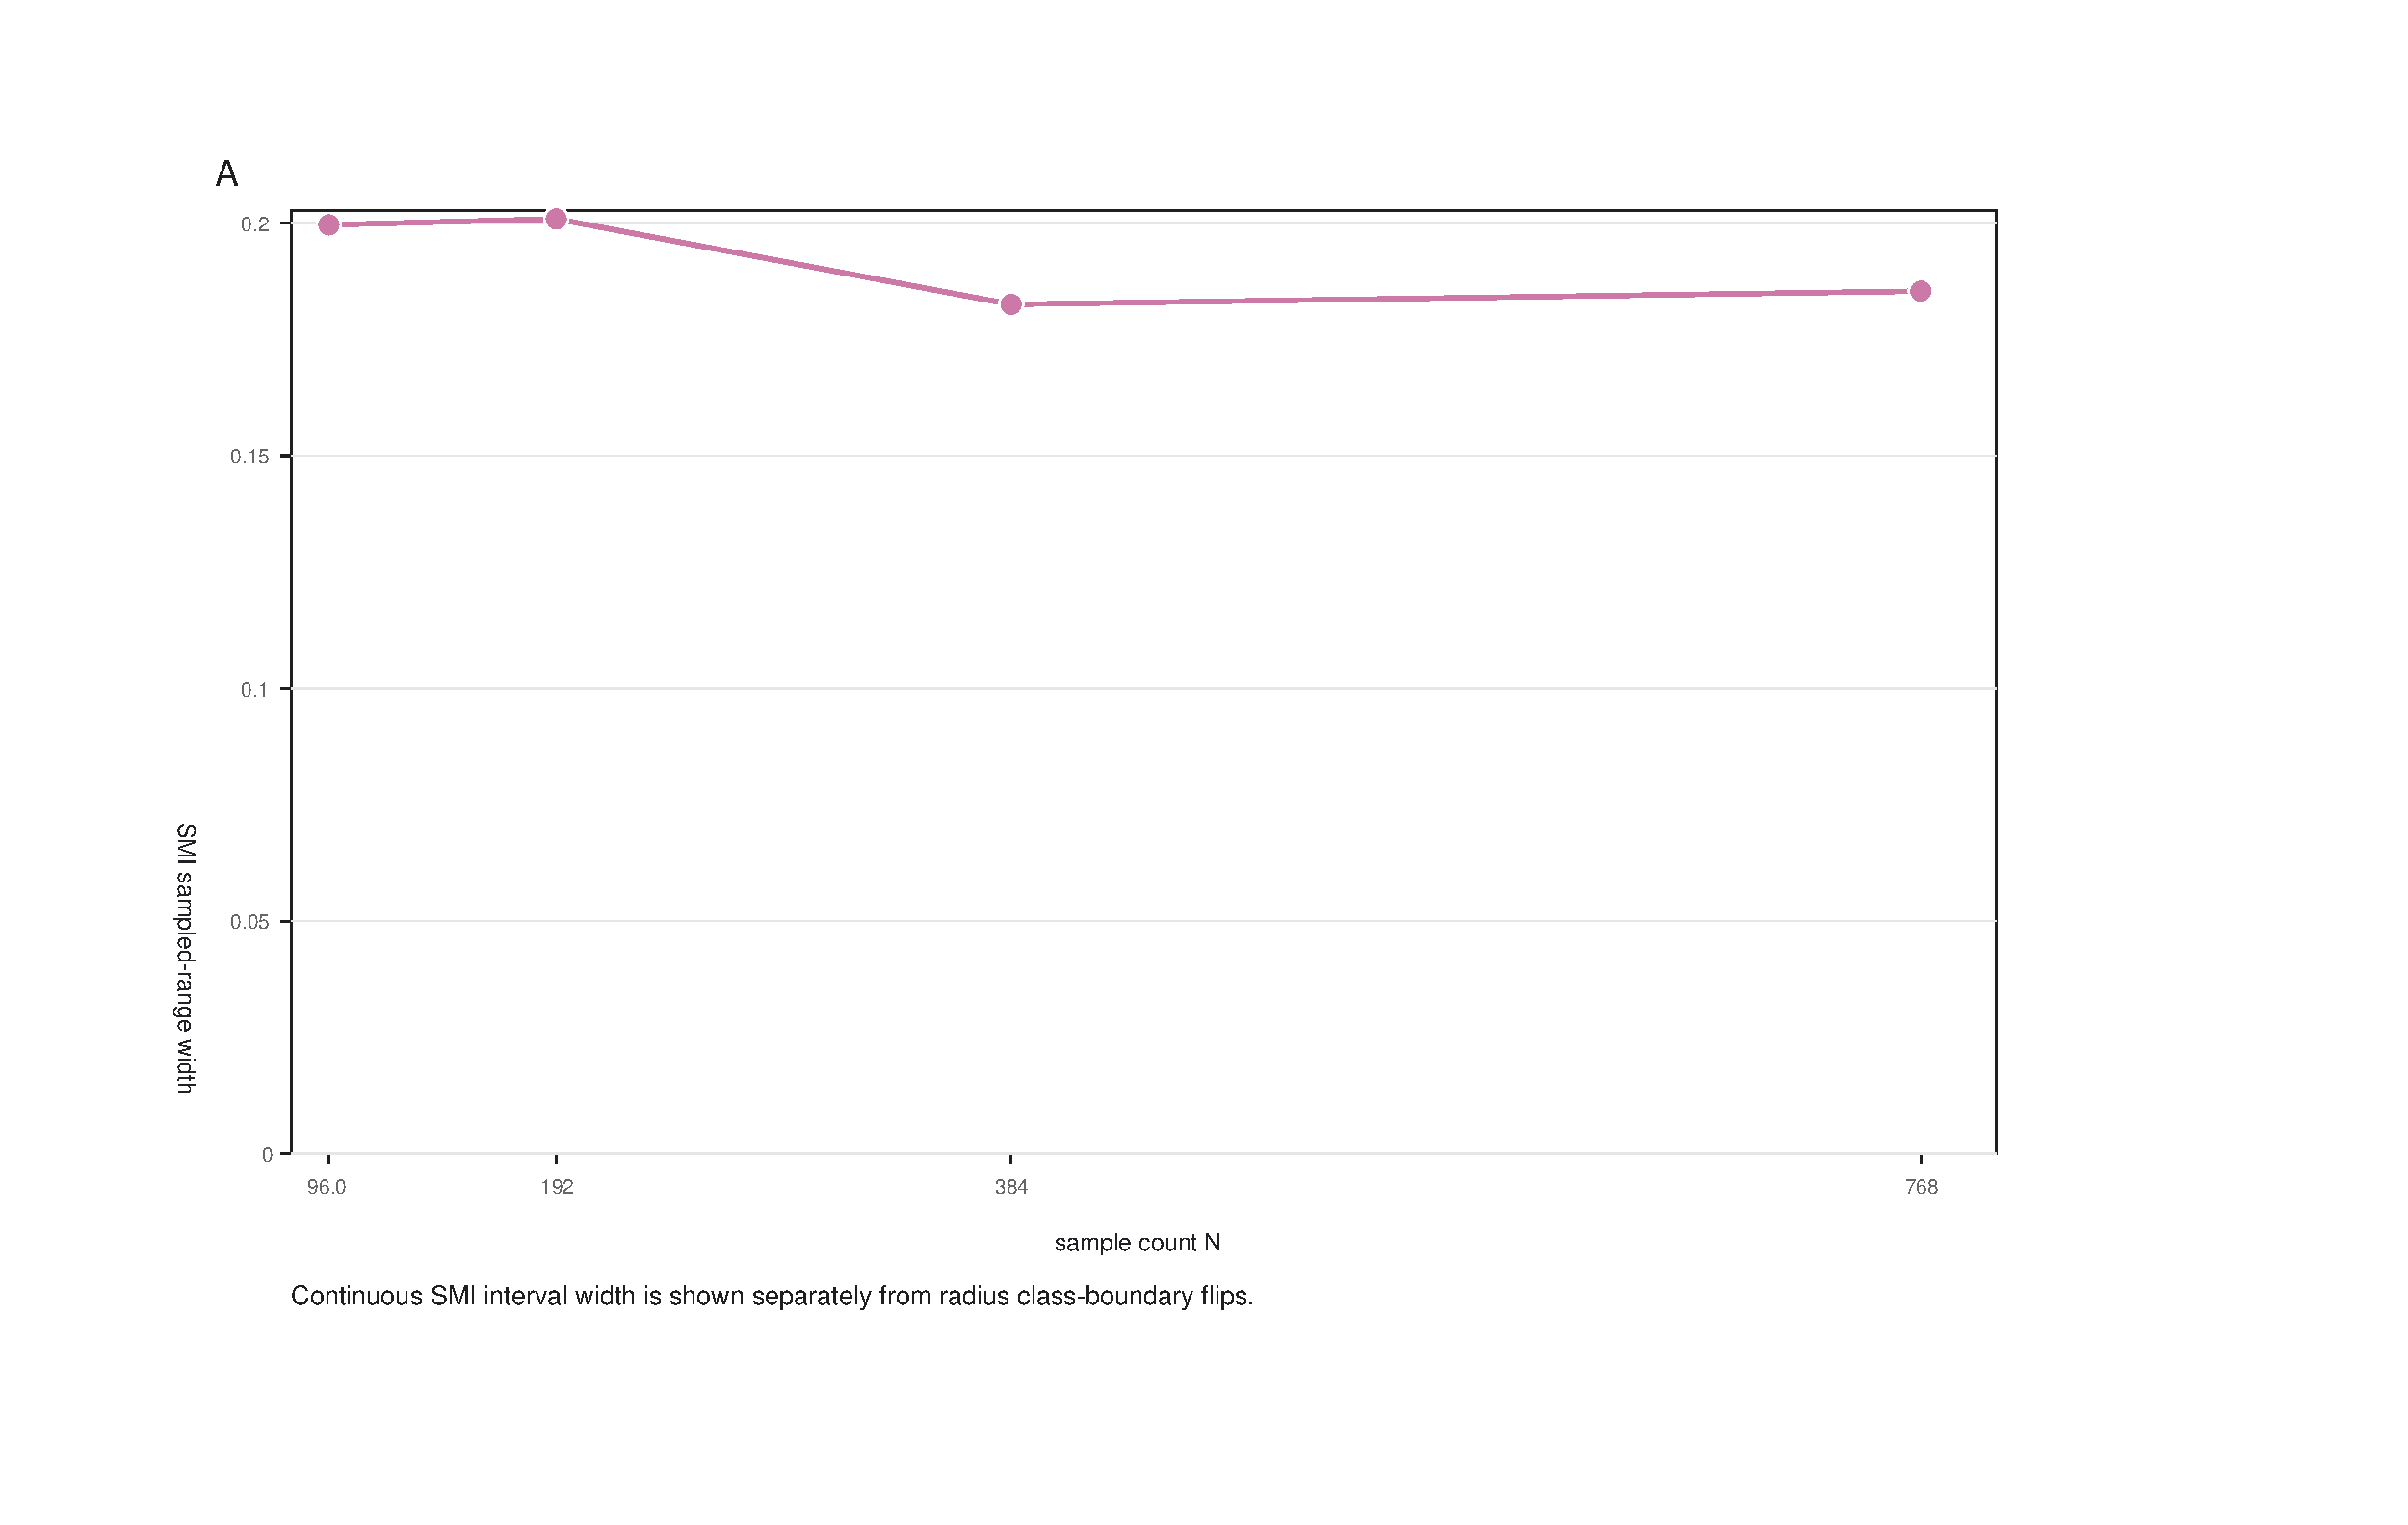
\includegraphics[width=0.85\textwidth,keepaspectratio]{../figures_publication/FigS5_smi_interval_width.pdf}
\caption{\textbf{Figure S5.} Continuous SMI uncertainty-width convergence across progressive sample counts. This continuous-width check complements the main-text radius class-flip design fraction.}
\label{fig:s5_interval}
\end{figure}
